\chapter{機率、資訊與熵}

\lectureoverview{統計力學始於微觀定律與不完備知識交會之處。我們先明確定義機率，再探討確定性運動本身如何賦予機率、守恆定律如何劃分狀態空間，以及為何保留資訊的動力學自然導向熵。等這套架構建立起來之後，才會談到第一定律與第零定律。}

\section{為什麼需要統計力學？}

統計力學有時被稱為舊物理學。這種說法沒有抓住重點。它既屬於前現代，也屬於現代，而且很可能在任何承接我們現有理論的後現代物理學中繼續發揮作用。具體模型不斷更迭；熱力學第二定律卻一再經受考驗，持續為我們指引方向。每當某種自然描述看似能憑空創造秩序、從根本上抹除資訊，或使封閉系統走向不自然的簡單狀態，第二定律便提醒我們：其中必定遺漏了某些因素。

這門學科或許不如新發現的粒子那樣引人注目，卻至少同樣深刻，而且普遍得多。氣體、液體、固體、輻射、黑洞、資訊和量子場，都需要統計推理。事實上，若不了解統計力學，就無法理解用來發現粒子的實驗設備。這也就是為什麼一代又一代傑出的物理學家，即使主要研究其他領域，也都精通統計力學：它不只實用，而且格外優美。

要了解為什麼需要統計力學，可以先從力學所提供的理想情形談起。封閉系統可以是我們所考慮的整個宇宙，也可以是隔離得足夠完善、因而不受周遭環境影響的子系統。如果知道它的初始條件和演化定律，經典力學便能給出完整的預測。量子力學改變了可預測的內容，但同樣具有明確定義的狀態，以及一條能預測該理論所容許最大資訊的定律。

原則上能夠預測，與實際上能夠理解，兩者相差甚遠。若列出這個房間裡每個分子的位置和速度，清單將長得驚人，幾乎立刻就會改變，而且幾乎回答不了我們真正關心的問題。因此，精確的微觀定律可以同時完全具備預測力，卻在實際應用上毫無用處。

統計力學是將機率論應用於這種物理情境。當初始條件無法完全精確得知、定律只能近似得知、系統是開放的，或單純因為微觀變數多到無法追蹤時，統計力學就不可或缺。這些情況都不代表預測能力薄弱。大量元素往往反而讓統計預測變得極為精確。

考慮一個孤立的氣體盒子。我們無法預測每個分子的軌跡，但只要少數宏觀資料，就能高精度地預測壓力、能量和許多其他宏觀量。仍然無法確定的是漲落。在某個不可預測的時刻，一小塊區域裡的分子可能多於平均值，而另一塊則可能少於平均值。這種事件落在機率分佈的尾端：機率低，但並非不可能。我們可以計算這類漲落應出現的頻率，卻無法預測某一次漲落會在什麼時刻發生。

擲硬幣也呈現相同的區別。公平地擲十億次，正面和反面的次數會相當接近。只要擲得夠多次，終究會出現一連串正面；但機率論預測的是它出現的頻率，而不是事先指定它何時發生。統計力學是為元素太小、太多，或兩者兼具的系統而設的。

本課程將介紹這些定律，以及它們在物質上的應用。這門學科值得反覆研習：學會之後，可能忘掉其中一些部分，再重新學習時，便會更深刻地體會哪些觀念才是根本。我們先從支配後續一切內容的觀念談起。

\section{作為基本語言的機率}

機率為何有效，並不是機率演算本身所能解釋的。機率預測可能在某一次試驗中失準；可能發生卻不太可能發生的結果，正是這個意思。理論告訴我們例外如何分佈，但不會讓例外消失。因此，我們把機率視為基本概念，並列出它所遵循的規則。

\subsection{狀態與歸一化}

令\(i\)表示一個可能的結果或系統的一種可能狀態。對一枚硬幣而言，\(i\)可以表示正面或反面。對一顆骰子而言，它可以從\(1\)到\(6\)。對兩顆骰子而言，一對指標可以記錄兩顆骰子的點數。我們先考慮有限的離散狀態空間，
\begin{equation}
 i=1,\ldots,N,
\end{equation}
之後再推廣到無限多個狀態，以及連續的狀態。

無知不代表系統沒有狀態，而是代表我們不知道它處於哪個狀態，因此對每種可能性都指定一個機率\(p_i\)。基本規則如下：
\begin{align}
 p_i &\geq 0, \label{eq:sm1-prob-positive}\\
 \sum_{i=1}^{N}p_i &=1. \label{eq:sm1-prob-normalization}
\end{align}
各種可能性彼此互斥，而且涵蓋所有情形：其中恰好有一種會發生。這裡不會有負機率，機率總和為一，因為某個允許的結果必定會發生。

\subsection{頻率與大數定律}

機率透過重複試驗與實驗相連。假設同一實驗進行\(N_{\mathrm{trials}}\)次，令\(N(i)\)表示結果\(i\)出現的試驗次數。頻率詮釋如下：
\begin{equation}
 p_i=
 \lim_{N_{\mathrm{trials}}\to\infty}
 \frac{N(i)}{N_{\mathrm{trials}}}.
 \label{eq:sm1-frequency}
\end{equation}
這是一項以理想極限表達的物理假設。沒有實驗室能進行無限多次實驗。這項主張是：試驗次數足夠多時，比值會穩定在足夠接近\(p_i\)的範圍內，以符合預期的預測。有限樣本的頻率會在極限值附近漲落。

\subsection{平均值}

現在為每個狀態指定一個數值\(f(i)\)。它可以是能量、動量，或任何我們想測量的量。其期望值為
\begin{equation}
 \langle f\rangle=\sum_i f(i)p_i.
 \label{eq:sm1-expectation}
\end{equation}
即使在量子力學之外，使用括號記號也很方便。以頻率來表示，同一個平均值為
\begin{equation}
 \langle f\rangle
 =
 \lim_{N_{\mathrm{trials}}\to\infty}
 \frac{1}{N_{\mathrm{trials}}}
 \sum_i f(i)N(i).
 \label{eq:sm1-frequency-average}
\end{equation}

對一枚硬幣，定義
\begin{equation}
 f(\mathrm{H})=+1,
 \qquad
 f(\mathrm{T})=-1.
\end{equation}
若正面和反面的機率各為\(1/2\)，則
\begin{equation}
 \langle f\rangle
 =(+1)\frac12+(-1)\frac12=0.
\end{equation}
平均值不一定是可能出現的結果。硬幣不會落在零上；零只是概括了兩種可能取值的分佈。

這段簡短的插曲確立了本學科通篇使用的詞彙：狀態、機率、頻率和期望值。

\section{指定機率的三種方式}

\subsection{對稱性}

為什麼我們通常給硬幣的兩面相同的機率？第一個答案是對稱性。翻轉一枚近乎理想的硬幣，正面和反面會互換，但實驗本身不變。因此，沒有物理理由偏向任何一種結果。真實的標記或瑕疵會引入微小偏差，但對稱模型足以描述我們所設想的實驗：
\begin{equation}
 p(\mathrm{H})=p(\mathrm{T})=\frac12.
\end{equation}

同樣的推理也會給對稱骰子的每一面指定機率\(1/6\)。更一般地說，除非有額外資訊打破對稱性，否則由對稱性相互關聯的構型會被指定相同的機率。

\subsection{實驗}

形狀不規則的骰子沒有能互換全部六面的對稱性。在這種情況下，光靠對稱性無法得出答案。或許有更深入的力學模型能預測偏差；但若沒有這樣的模型，誠實的做法就是進行實驗：多次擲骰，記錄頻率，等頻率趨於穩定，再用所得的機率表進行後續預測。

對稱性和實驗並非互相競爭的定義，而是取得機率分佈資訊的兩種途徑。統計力學會大量運用對稱性，而動力學則提供第三種途徑。

\subsection{從確定性運動得出機率}

想像一個不規則物體，有六種不同顏色的構型。它依照確定的更新規則，每隔固定的離散時間改變一次狀態：
\begin{equation}
 R\longrightarrow B\longrightarrow Y\longrightarrow G
 \longrightarrow O\longrightarrow P\longrightarrow R.
 \label{eq:sm1-six-cycle}
\end{equation}
物體本身不必具有任何幾何對稱性。這條規則只說明某個構型之後會接續哪個構型。

\begin{figure}[htbp]
\centering
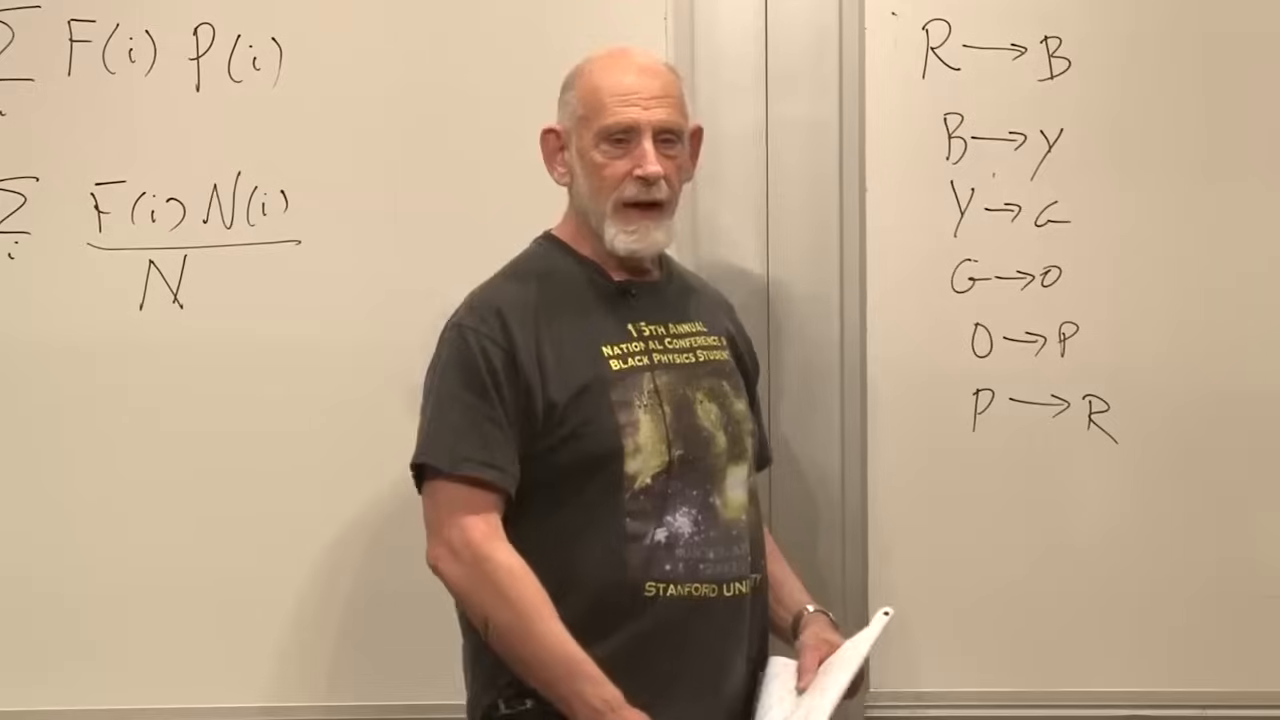
\includegraphics[width=0.92\textwidth]{lecture_01_figure_02.png}
\caption{左側黑板保留期望值公式，右側則列出六種顏色狀態的確定性更新規則。}
\lectureframe{00:26:28}
\end{figure}

若將黑板上的列表畫成有向迴圈，關係會更清楚：
\begin{figure}[htbp]
\centering
\begin{tikzpicture}[
  >=Latex,
  state/.style={draw,circle,minimum size=8mm,inner sep=1pt}
]
\node[state] (R) at (90:2.2) {$R$};
\node[state] (B) at (30:2.2) {$B$};
\node[state] (Y) at (-30:2.2) {$Y$};
\node[state] (G) at (-90:2.2) {$G$};
\node[state] (O) at (-150:2.2) {$O$};
\node[state] (P) at (150:2.2) {$P$};
\draw[->] (R) -- (B);
\draw[->] (B) -- (Y);
\draw[->] (Y) -- (G);
\draw[->] (G) -- (O);
\draw[->] (O) -- (P);
\draw[->] (P) -- (R);
\end{tikzpicture}
\caption{一個由六個狀態組成的單一軌道。每個週期中，每種狀態都會經過一次。}
\label{fig:sm1-six-cycle}
\end{figure}

假設我們不知道初始狀態，並在未知時刻拍下一張快照。由於每一步持續時間相同，系統在每種顏色狀態停留的時間都是一個週期的六分之一：
\begin{equation}
 p(R)=p(B)=p(Y)=p(G)=p(O)=p(P)=\frac16.
 \label{eq:sm1-uniform-cycle}
\end{equation}
這種均等並非來自物體的形狀，而是來自系統在各狀態中停留的時間相同。

我們可以重新排列箭頭，形成一條不同的微觀定律，但仍然是一個由六個狀態組成的迴圈。狀態的先後順序改變了，但快照機率仍是\(1/6\)，因為每個週期中仍會經過每種狀態一次。因此，這項預測既不需要知道起點，也不需要知道具體的先後順序；只要知道軌道結構，以及每次更新所對應的時間相同即可。

\begin{classroomqa}
\classquestion{如果物體並不對稱，給每種顏色指定機率\(1/6\)，在什麼意義上才合理？}
\lecturerresponse{這種指定依據的是動力學，而不是幾何。若在六步軌道的未知相位拍下快照，取樣的就是六個等長的時間區間。相關的等價性存在於軌道上的各個位置之間，而不在物體的各面之間。若停留時間不相等，機率也會不相等。
\lecturetimestamp{00:27:11--00:29:49}}
\end{classroomqa}

\section{不連通的迴圈與守恆量}

確定性定律不一定會讓所有狀態都落在同一條軌道上。考慮兩條彼此不連通的迴圈：
\begin{equation}
 R\longrightarrow B\longrightarrow G\longrightarrow R,
 \qquad
 P\longrightarrow Y\longrightarrow O\longrightarrow P.
 \label{eq:sm1-two-cycles}
\end{equation}
如果知道系統位於第一條迴圈上，那麼
\begin{equation}
 \begin{aligned}
 p(R)=p(B)=p(G)&=\frac13,\\
 p(P)=p(Y)=p(O)&=0.
 \end{aligned}
\end{equation}
若知道它位於第二條迴圈上，則上述機率指定會對調。

更一般的情況需要指定先驗權重。將兩條迴圈標記為\(+1\)和\(-1\)，並令它們的機率分別為\(p_+\)和\(p_-\)，且滿足
\begin{equation}
 p_++p_-=1.
\end{equation}
則有
\begin{align}
 p(R)=p(B)=p(G)&=\frac{p_+}{3},\\
 p(P)=p(Y)=p(O)&=\frac{p_-}{3}.
 \label{eq:sm1-sector-weights}
\end{align}
因子\(1/3\)來自迴圈內的運動，數值\(p_+\)和\(p_-\)則不是。這些數值必須來自額外資訊，例如另一項實驗，或另一個能選定初始扇區的系統。

標記\(+1\)和\(-1\)定義了一個守恆量：系統一旦從其中一條迴圈出發，更新規則就絕不會把它帶到另一條迴圈。可以把這個量稱為能量，也可以用\emph{zilch}這類暫名來稱呼它。名稱並不重要。守恆表示狀態空間被劃分為動力學無法跨越的區域。

兩條迴圈包含的狀態數目不必相同。四狀態軌道和二狀態軌道仍然構成兩個守恆扇區。以時間取樣時，第一個扇區內各狀態的機率為\(1/4\)，第二個扇區內各狀態的機率為\(1/2\)；兩者各自還要乘上所在扇區的先驗機率。因此，統計力學必須回答兩個在邏輯上彼此獨立的問題：
\begin{enumerate}
\item 給定一個守恆扇區後，動力學在其中各個狀態停留多久？
\item 應該給守恆扇區本身指定什麼機率？
\end{enumerate}

\begin{classroomqa}
\audiencequestion{我們是否假設同一守恆扇區內的所有狀態都具有相同機率？}
\lecturerresponse{對於這裡展示的離散玩具模型，答案是肯定的，因為每個狀態持續的時間相同，且運動是確定性的。我們不知道的是軌道的初始相位。毫秒級的計時偵測器無法分辨微秒級的更新，但足夠快速的快照仍能辨識當下捕捉到的狀態。在更一般的系統中，必須明確納入不相等的停留時間。
\lecturetimestamp{00:36:16--00:37:17}}
\end{classroomqa}

\begin{classroomqa}
\audiencequestion{如果拍下兩張快照，而第一張辨識出系統位於某條迴圈上，那麼第二張是否也應辨識出同一條迴圈？}
\lecturerresponse{是的，這正是守恆的意義。測量一旦確定守恆量的值，就可以根據該值來條件化未來的機率，而另一個扇區內各狀態的機率則為零。
\lecturetimestamp{00:37:18--00:37:45}}
\end{classroomqa}

\subsection{兩個系統之間的能量共享}

現在把抽象標記換成能量。一個孤立的盒子是封閉系統，其能量守恆。兩個互不作用的孤立盒子，各自的能量分別守恆。若用一條可讓能量流動的狹窄通道將它們連接起來，各自的能量就可能改變，但總能量仍然固定。

\begin{figure}[htbp]
\centering
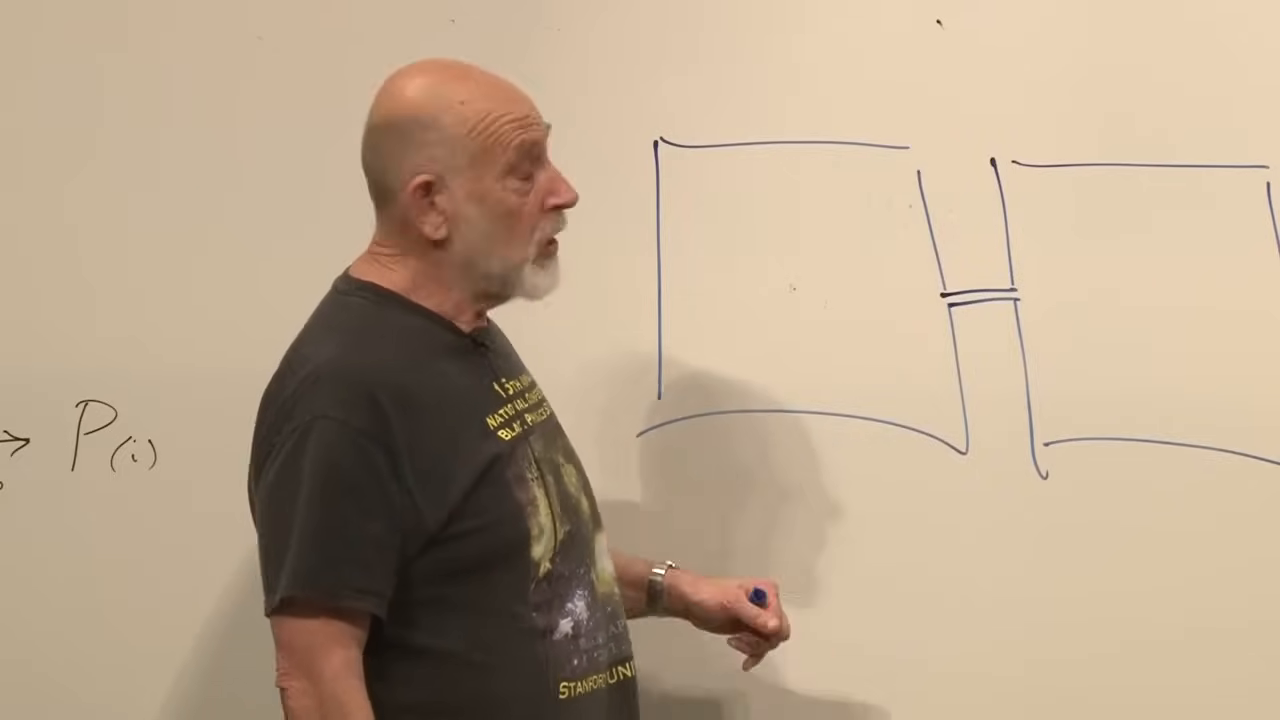
\includegraphics[width=0.92\textwidth]{lecture_01_figure_03.png}
\caption{兩個子系統由一條狹窄通道連接，能量可以經由通道流動。}
\lectureframe{00:39:19}
\end{figure}

\begin{figure}[htbp]
\centering
\begin{tikzpicture}[>=Latex]
\draw[thick,rounded corners=4pt] (-4,1.8) rectangle (-0.7,-1.5);
\draw[thick,rounded corners=4pt] (0.7,1.5) rectangle (4,-1.8);
\draw[thick] (-0.7,0.45) -- (0.7,0.45);
\draw[thick] (-0.7,-0.35) -- (0.7,-0.35);
\draw[<->,very thick] (-0.45,0.05) -- (0.45,0.05);
\node at (-2.35,0.15) {subsystem \(1\)};
\node at (2.35,-0.15) {subsystem \(2\)};
\node[above] at (0,0.5) {energy exchange};
\end{tikzpicture}
\caption{連接一旦打開，只有\(E_1+E_2\)守恆。能量如何分配便成為機率問題。}
\label{fig:sm1-connected-systems}
\end{figure}

給定總能量後，我們可以問：子系統\(1\)具有\(E_1\)、而子系統\(2\)具有其餘能量的機率是多少。相同的盒子，平均而言應具有相同能量，但平均值並不能描述完整的分佈。因此，要決定某個子系統的機率，一種方法是將它置於更大的封閉系統中，由該系統的守恆定律補足缺少的資訊。這種建構方式將在統計力學中反覆出現。

\section{好定律、壞定律與負第一定律}

並非每一種確定性更新規則都適合作為基本定律。考慮以下映射：
\begin{equation}
 \begin{aligned}
 R&\mapsto R,& B&\mapsto R,& Y&\mapsto R,\\
 G&\mapsto R,& O&\mapsto R,& P&\mapsto R.
 \end{aligned}
 \label{eq:sm1-all-to-red}
\end{equation}
它能完美預測未來：一步之後，狀態就是紅色。但它無法反向預測。一旦系統處於紅色，就無從得知它原先是藍色、黃色、綠色、橙色、紫色，還是紅色。

\begin{figure}[htbp]
\centering
\begin{tikzpicture}[
  >=Latex,
  state/.style={draw,circle,minimum size=8mm,inner sep=1pt}
]
\node[state,fill=red!12] (R) at (0,0) {$R$};
\node[state] (B) at (-3,1.6) {$B$};
\node[state] (Y) at (-3,0) {$Y$};
\node[state] (G) at (-3,-1.6) {$G$};
\node[state] (O) at (3,1.6) {$O$};
\node[state] (P) at (3,-1.6) {$P$};
\draw[->] (B) -- (R);
\draw[->] (Y) -- (R);
\draw[->] (G) -- (R);
\draw[->] (O) -- (R);
\draw[->] (P) -- (R);
\draw[->,loop above] (R) to (R);
\end{tikzpicture}
\caption{多對一的定律能預測下一個狀態，卻抹除了不同可能過去狀態之間的差異。}
\label{fig:sm1-bad-law}
\end{figure}

相較之下，閉合迴圈會保留這些差異。只要知道經過的時間，即使已過了數千個週期，我們仍能將狀態向前或向後演化。這條定律保留了不同初始條件之間的差異。Susskind 將這項要求稱為\emph{物理學的負第一定律}：資訊不會從根本上丟失。

對有限的離散狀態空間而言，圖示判準很簡單：
\begin{quote}
良好的定律中，每個狀態都恰好有一條向外箭頭，也恰好有一條指向它的箭頭。
\end{quote}
向外的箭頭決定未來；指向該狀態的箭頭則能重建過去。從數學上看，更新就是對狀態作置換。

\subsection{摩擦只是表面上的反例}

連續情形下的對應定理是劉維爾定理。摩擦看似與它矛盾。把橡皮擦在桌面上滑動，無論從哪裡開始，它最終都會停下來。示意性的阻力方程為
\begin{equation}
 m\ddot x=-\gamma\dot x,
 \qquad \gamma>0.
 \label{eq:sm1-drag}
\end{equation}
速度會按指數衰減。如果這就是密閉房間中每個粒子的根本定律，所有運動都會消失，溫度會降到零，而許多初始狀態會合併成同一個最終狀態。能量守恆會失效，資訊會消失，無序度也會降低。這就是一切狀態都變成紅色的連續版本。

真實的摩擦並非如此。橡皮擦會使桌面、橡皮擦本身和周遭環境升溫。微觀位置與動量會記錄可見運動中消失的那些差異。摩擦方程是省略未觀測自由度後，對子系統所用的有效方程；它不是描述完整封閉系統的基本耗散定律。

\begin{classroomqa}
\classquestion{微分方程
\(m\ddot x=-\gamma\dot x\)代表什麼？為什麼它不是描述封閉系統的基本定律？}
\lecturerresponse{它描述黏滯阻力。若只看這條方程，每個速度都會趨近於零，這會使氣體不論初始溫度如何，最後都冷卻到零。在完整的封閉系統描述中，流失的機械能和資訊會轉移到微觀自由度中。只有在略去這些變數之後，阻力方程才可靠。
\lecturetimestamp{00:44:40--00:48:56}}
\end{classroomqa}

\section{佔據狀態與最初的熵}

資訊守恆也可以用機率來表述。假設\(M\)個狀態中有\(N\)個被指定相同的機率，
\begin{equation}
 p_i=
 \begin{cases}
 1/M, & i\text{ in the occupied set},\\
 0, & i\text{ outside it}.
 \end{cases}
 \label{eq:sm1-uniform-occupied}
\end{equation}
保留資訊的更新可以重新排列哪些狀態被佔據，卻不能將它們合併。之後每個時刻，仍有\(M\)個狀態的機率為\(1/M\)。相較之下，壞映射\eqref{eq:sm1-all-to-red}可以將許多已佔據的狀態合併成一個。

數值\(M\)衡量無知程度。若\(M=N\)，每個狀態都有可能，我們的無知程度達到最大。若\(M=1\)，微觀狀態便已完全確知。因此，熵的第一個定義是
\begin{equation}
 S=\log M.
 \label{eq:sm1-entropy-logm}
\end{equation}
由此可得
\begin{equation}
 S_{\max}=\log N,
 \qquad
 S_{\min}=0.
\end{equation}
若狀態空間無限大，就不一定存在有限上限。

在這套論述中，熵先於溫度出現，甚至早於能量守恆的正式陳述。從這個意義上說，熵更為基本。然而，熵並非力學系統本身單獨具有的性質；它同時取決於系統，以及代表已知資訊的機率分佈。資訊不同的觀察者，可能會對同一力學系統指定不同的熵。

在精確的微觀演化下，已佔據的狀態只是重新排列，因此這個細粒化熵守恆。實際上，我們會失去時間資訊、捨棄關聯性，也無法追蹤數量龐大的變數。於是，機率分佈會擴散到更多可能性上，粗粒描述所指定的熵也隨之增加。即使方程沒有破壞資訊，我們能運用的描述仍可能失去資訊。

\begin{classroomqa}
\classquestion{具有\(N\)個狀態的有限系統，其可能的最大熵是多少？}
\lecturerresponse{最大熵為\(\log N\)，在所有\(N\)個狀態的機率都相等時達到。最小熵為零，在其中一個狀態的機率為一時達到。因此，熵衡量的不只是可用的狀態空間，也包括我們掌握資訊的情形。
\lecturetimestamp{00:56:46--00:58:19}}
\end{classroomqa}

\section{連續相空間中的劉維爾流}

對於位置與動量都是連續變數的粒子，微觀狀態是相空間中的一個點。我們以\(q_a\)表示座標，以\(p_a\)表示其共軛動量。粒子數目很多時，相空間會有極多個軸；二維圖上只有一個\(q\)和一個\(p\)，只是用來代替完整相空間的示意圖。相空間的維度必為偶數，因為每個座標都有一個相對應的動量。

假設用一個區域\(\Omega_0\)來表示我們掌握的資訊：機率密度在區域內均勻，區域外則為零。例如，知道每個粒子都在房間裡，就會限制位置座標；限制粒子的速率，則會限制動量座標。

哈密頓演化會使相空間中的每個點沿著軌跡運動。彼此相鄰的點仍會移動到相鄰的位置，而佔據區域則像不可壓縮流體的一團流體般演化：
\begin{figure}[htbp]
\centering
\begin{tikzpicture}[>=Latex,scale=0.95]
\draw[->] (-4.2,0) -- (4.3,0) node[right] {$q$};
\draw[->] (-3.7,-2.2) -- (-3.7,2.4) node[above] {$p$};
\draw[fill=blue!12,thick]
  (-3.0,-0.5) .. controls (-2.7,1.0) and (-1.3,1.2) .. (-0.9,0.1)
  .. controls (-0.6,-1.0) and (-2.2,-1.4) .. cycle;
\node at (-1.9,0.0) {$\Omega_0$};
\draw[->,very thick] (-0.3,0.2) -- (0.8,0.2);
\draw[fill=orange!15,thick]
  (1.2,-1.1) .. controls (1.5,0.3) and (2.3,1.8) .. (3.2,1.1)
  .. controls (3.6,0.7) and (2.8,-0.4) .. (2.5,-1.5)
  .. controls (2.1,-1.8) and (1.5,-1.6) .. cycle;
\node at (2.35,0.1) {$\Omega_t$};
\end{tikzpicture}
\caption{哈密頓流可以拉伸並剪切佔據的相空間區域，但會保持其體積不變。}
\label{fig:sm1-liouville-flow}
\end{figure}

劉維爾定理指出：
\begin{equation}
 \operatorname{Vol}(\Omega_t)
 =
 \operatorname{Vol}(\Omega_0).
 \label{eq:sm1-liouville-volume}
\end{equation}
若初始密度在\(\Omega_0\)上均勻，輸運後的密度就會在\(\Omega_t\)上均勻。這相當於在連續情形中，佔據狀態的數目與權重都保持不變。

這項定理也以幾何方式解開了摩擦之謎。若只看橡皮擦的可見動量，一團可能狀態似乎會朝\(p=0\)收縮。但在完整相空間中，這團狀態會擴散到橡皮擦和桌上分子的位置與動量等變數中。投影可以收縮，完整的高維體積卻仍保持不變。

\begin{classroomqa}
\classquestion{如果每條可見軌跡都趨近靜止，佔據的相空間區域是否已收縮到\(p=0\)軸上？}
\lecturerresponse{只有在約化後的投影中才是如此。完整系統還包含桌子、橡皮擦和周遭環境的微觀變數。可見的動量範圍縮小時，分佈會擴散到那些隱藏方向。劉維爾定理適用於完整的封閉相空間，而不是不完整的宏觀變數集合。
\lecturetimestamp{01:04:37--01:06:29}}
\end{classroomqa}

\section{從負第一定律到第一定律}

\subsection{簡談第零定律}

在陳述第一定律之前，先介紹第零定律很有幫助。熱平衡尚未定義，因此目前這條定律只是一項結構性陳述：
\begin{quote}
若系統\(A\)與\(B\)處於熱平衡，且\(B\)與\(C\)處於熱平衡，那麼\(A\)與\(C\)也處於熱平衡。
\end{quote}
這種遞移性日後會讓溫度得以定義。目前先暫且擱置。

\subsection{能量守恆}

封閉系統的第一定律就是
\begin{equation}
 \frac{dE}{dt}=0.
 \label{eq:sm1-first-law}
\end{equation}
這個簡潔的形式隱藏了它的力量。能量是一種守恆量，而「能量」一詞日後還會獲得更多熱力學上的意涵。

如果封閉系統由兩部分組成，而且兩部分的能量可以相加，
\begin{equation}
 E=E_1+E_2,
\end{equation}
那麼
\begin{equation}
 \frac{dE_1}{dt}+\frac{dE_2}{dt}=0,
 \qquad\text{or}\qquad
 \frac{dE_1}{dt}=-\frac{dE_2}{dt}.
 \label{eq:sm1-energy-exchange}
\end{equation}
第二種形式清楚表明能量如何交換：一個子系統失去的能量，會由另一個子系統獲得。

可加性假設需要審慎看待。兩個互相吸引的粒子各有動能，但它們的交互作用也會帶來一份屬於兩者整體的位能。總能量守恆，儘管它無法精確地寫成一個物體的能量加上另一個物體的能量。

熱力學往往可以採用極佳的可加近似，因為整體能量隨體積增加，而大型相鄰部分之間的短程交互作用能，主要隨接觸面積增加。把一張大桌子分成幾塊：每塊的內能取決於體積，而相鄰桌塊間的耦合則取決於接觸面。桌塊夠大時，後者相對較小。方程\eqref{eq:sm1-first-law}對整個封閉系統而言是精確的；子系統的形式\eqref{eq:sm1-energy-exchange}則假設交互作用能可以忽略。

\begin{classroomqa}
\audiencequestion{歸一化條件\(\sum_i p_i=1\)是否也假設列出的結果彼此互斥？}
\lecturerresponse{是的。狀態標籤的定義要求各種可能性彼此不重疊：骰子若處於黃色狀態，就不會同時處於紅色狀態。日常用語中顏色可以混合，但機率計算所採用的狀態劃分，必須由互斥的可能性構成。
\lecturetimestamp{01:12:14--01:12:55}}
\end{classroomqa}

\section{回到熵}

講課現在明確回到尚未處理完的問題。溫度雖然是感官熟悉的量，卻是推導而來的量。要明確定義溫度，必須先確立熵與能量的概念。

\subsection{一般機率分佈}

特殊定義\(S=\log M\)適用於\(M\)個狀態等機率、其他狀態的機率皆為零的情況。一般分佈不必是矩形的；各狀態標籤所對應的權重，可以平滑或不規則地變化。

\begin{figure}[htbp]
\centering
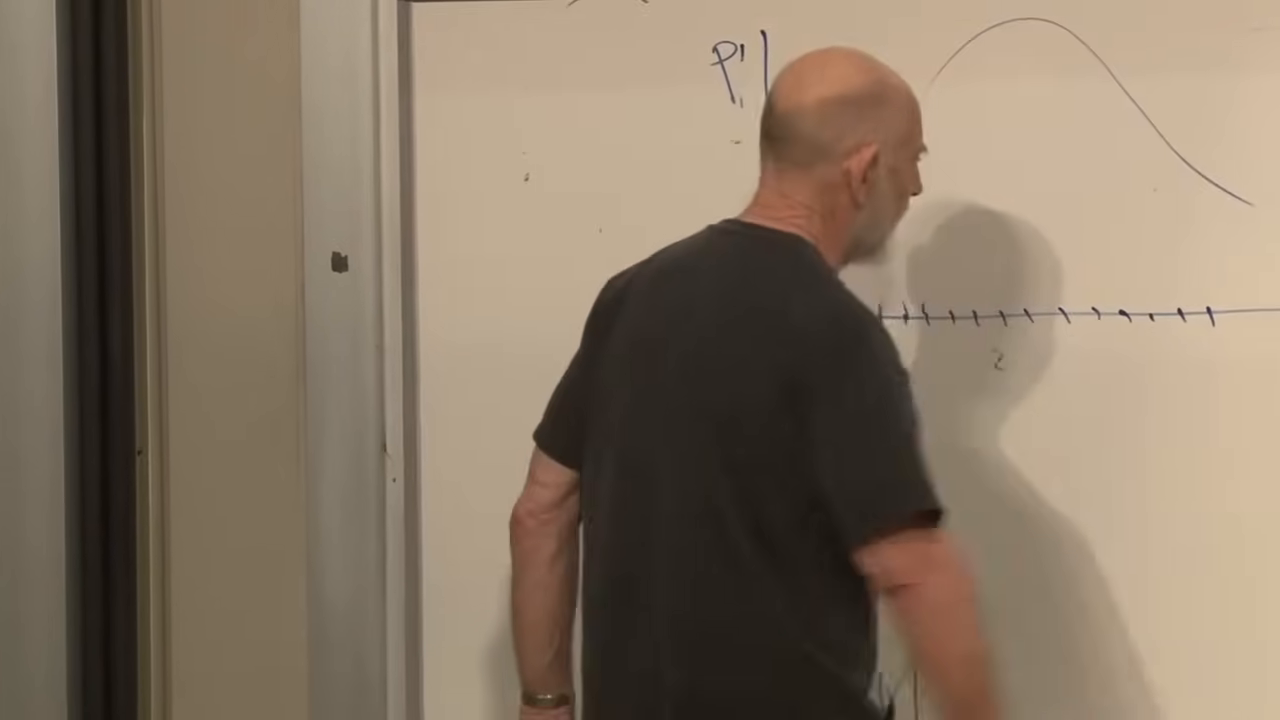
\includegraphics[width=0.92\textwidth]{lecture_01_figure_05.png}
\caption{繪於離散狀態標籤上的機率分佈。熵所需衡量的是分佈的展寬，而不是曲線的精確形狀。}
\lectureframe{01:14:40}
\end{figure}

\begin{figure}[htbp]
\centering
\resizebox{\linewidth}{!}{%
\begin{tikzpicture}[>=Latex,scale=0.93]
\draw[->] (-4.2,0) -- (4.4,0) node[right] {state label \(i\)};
\draw[->] (-4,0) -- (-4,3.2) node[above] {$p_i$};
\foreach \x in {-3.6,-3.1,...,3.6}
  \draw (\x,0.08) -- (\x,-0.08);
\draw[very thick]
  plot[smooth] coordinates {
  (-3.7,0.12) (-3.0,0.28) (-2.3,0.72) (-1.6,1.45)
  (-0.9,2.25) (-0.2,2.65) (0.5,2.28) (1.2,1.55)
  (1.9,0.88) (2.7,0.38) (3.5,0.14)};
\draw (-1.8,-0.18) -- (-1.8,-0.5);
\draw (1.8,-0.18) -- (1.8,-0.5);
\draw[<->] (-1.8,-0.46) -- (1.8,-0.46);
\node at (0,-0.82) {effective spread};
\end{tikzpicture}
}
\caption{窄分佈的不確定性小於寬分佈。熵必須衡量整個分佈。}
\label{fig:sm1-probability-spread}
\end{figure}

一般定義為
\begin{equation}
 S=-\sum_i p_i\log p_i.
 \label{eq:sm1-shannon-entropy}
\end{equation}
利用\eqref{eq:sm1-expectation}，可寫成
\begin{equation}
 S=-\langle\log p\rangle.
\end{equation}
負號是為了補償\(\log p_i<0\)（當\(0<p_i<1\)時）這一點。

\subsection{恢復均勻分佈的結果}

我們必須檢查一般公式是否能重現第一個定義。對於未佔據的狀態，\(p_i=0\)，而\(\log p_i\)會發散。兩者的乘積有明確的極限值
\begin{equation}
 \lim_{p\to0^+}p\log p=0.
 \label{eq:sm1-plogp-limit}
\end{equation}
因此，機率為零的狀態不會有任何貢獻。

\begin{classroomqa}
\audiencequestion{如果\(p_i=0\)，該項真的會消失嗎？零的對數是負無窮。}
\lecturerresponse{該項由極限\(\lim_{p\to0^+}p\log p\)定義，其值為零。因子\(p\)趨近於零的速度比對數發散的速度快。因此，機率任意小的狀態所作的貢獻也任意小，而機率恰為零的狀態則毫無貢獻。
\lecturetimestamp{01:18:27--01:19:46}}
\end{classroomqa}

對於\(M\)個佔據狀態中的每一個，都有\(p_i=1/M\)。因此
\begin{align}
 S
 &=-\sum_{\mathrm{occupied}\ i}
 \frac1M\log\!\left(\frac1M\right)\\
 &=-M\frac1M\log\!\left(\frac1M\right)\\
 &=-\log\!\left(\frac1M\right)
 =\log M.
 \label{eq:sm1-entropy-check}
\end{align}
一般表示式與特殊情況下的表示式完全一致。較寬廣的分佈會讓更多選項具有可觀的權重，因此熵較大；較集中的分佈則有較小的熵。

\begin{figure}[htbp]
\centering
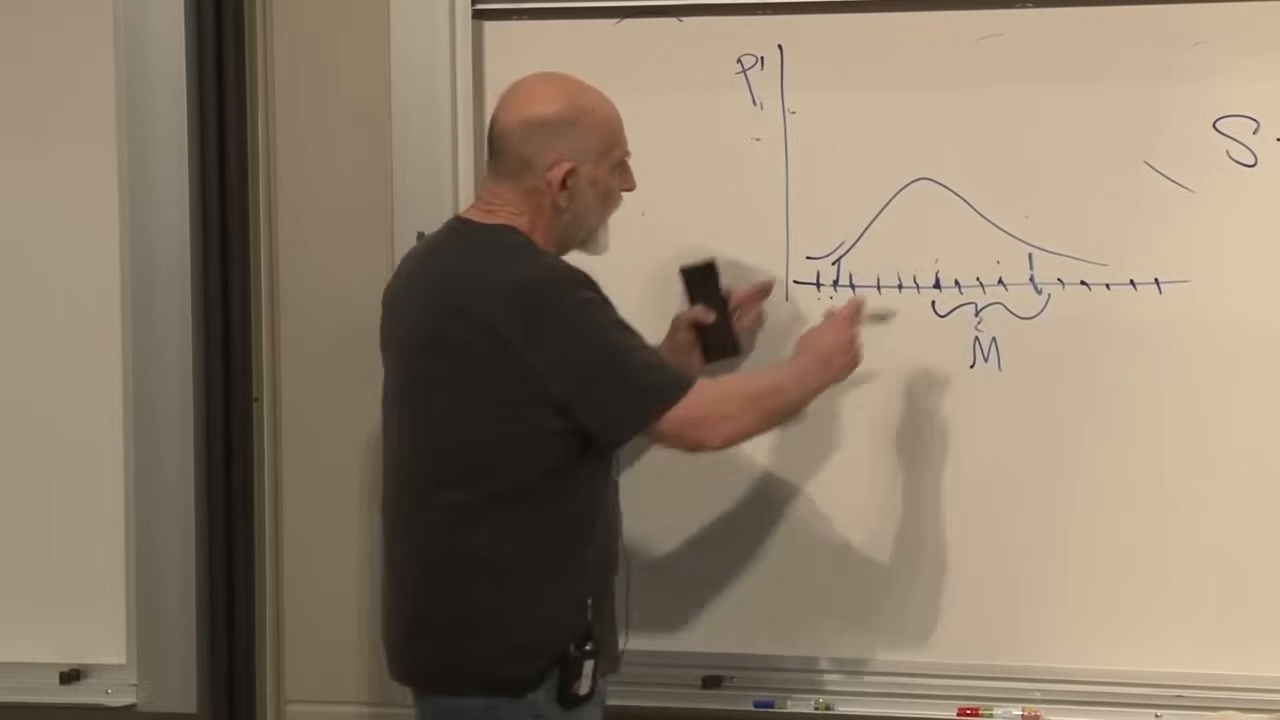
\includegraphics[width=0.92\textwidth]{lecture_01_figure_06.png}
\caption{圖中標示的寬度\(M\)突顯了顯著機率的分布範圍與熵之間的關聯。}
\lectureframe{01:16:42}
\end{figure}

熵屬於狀態空間上的機率分佈。它不是像單一微觀態的能量或動量那樣的單一可觀測量。精確狀態可以用集中在該狀態上的分佈表示，此時熵為零；但當我們掌握的資訊改變時，熵也會改變。

\section{硬幣、位元與明確計數}

令\(n\)為硬幣數目。微觀構型的數目為
\begin{equation}
 N=2^n.
 \label{eq:sm1-coin-state-count}
\end{equation}
如果我們對硬幣一無所知，所有\(2^n\)種構型的機率都相同，因此
\begin{equation}
 S_{\max}=\log(2^n)=n\log2.
 \label{eq:sm1-coin-max-entropy}
\end{equation}
熵會隨獨立硬幣的數目相加。

以\(2\)為底的對數下，完全未知的二態系統具有一位元的熵；以自然對數計算時，其熵為\(\log2\)。單位是約定俗成的；底層的排序與可加性不受影響。

在另一個極端，如果每枚硬幣的狀態都已知，就恰好只有一種構型的機率為一：
\begin{equation}
 S=0.
\end{equation}
掌握的資訊越多，熵就越小。

現在假設\(n\)枚硬幣中恰有一枚是反面，其餘都是正面，但反面的位置未知。共有\(n\)種等可能的構型，分別對應反面可能出現的位置，因此
\begin{equation}
 S=\log n.
 \label{eq:sm1-one-tail-entropy}
\end{equation}
這通常不是\(\log2\)的整數倍。位元是方便使用的單位，並不表示所有熵值都以整數位元為間隔。

\begin{classroomqa}
\audiencequestion{\(\log2\)的出現僅僅是因為每枚硬幣有兩種可能狀態嗎？如果一個元素有三種可能狀態，熵會是\(\log3\)嗎？}
\lecturerresponse{正是如此。一個有\(k\)種可能狀態、且各狀態均勻未知的元素，貢獻\(\log k\)。二元開關在電腦中特別方便，因為實體開關自然能實現兩種穩定狀態，而且二是最小的非平凡整數。
\lecturetimestamp{01:29:55--01:30:48}}
\end{classroomqa}

\begin{classroomqa}
\audiencequestion{對數的底數是什麼？}
\lecturerresponse{在這些物理公式中，\(\log\)表示自然對數。資訊理論學者常用底數\(2\)，因此熵直接以位元為單位。改變底數會讓所有熵值乘上一個固定的換算因子，但不會改變任何物理結論。
\lecturetimestamp{01:30:49--01:32:06}}
\end{classroomqa}

\section{連續相空間中的熵}

回到經典相空間\(\Gamma\)。如果機率密度在體積為\(V_\Gamma\)的區域內均勻分布，區域外則為零，那麼，這相當於計數\(M\)個等可能狀態：
\begin{equation}
 S=\log\!\left(\frac{V_\Gamma}{V_0}\right).
 \label{eq:sm1-continuous-uniform}
\end{equation}
這裡的\(V_\Gamma\)是座標與動量所構成的完整高維空間中的體積，不是一般的空間體積。固定體積\(V_0\)是參考相空間元，用來使對數的引數成為無因次量。令\(V_0=1\)，便得到黑板上使用的簡寫\(S=\log V_\Gamma\)。

對於一般的機率密度\(P(q,p)\)，離散求和會變成相空間積分。歸一化條件為
\begin{equation}
 \int_\Gamma d\Gamma\,P(q,p)=1,
 \label{eq:sm1-continuous-normalization}
\end{equation}
熵則為
\begin{equation}
 S=-\int_\Gamma d\Gamma\,
 P(q,p)\log\!\bigl[P(q,p)V_0\bigr].
 \label{eq:sm1-continuous-entropy}
\end{equation}
此密度表示每個相空間元中的機率。概念上，\eqref{eq:sm1-continuous-entropy}仍衡量機率分布得有多廣；若分布均勻於一個區域，其熵便化為佔據體積以參考相空間元為單位計算所得的對數。改變這個固定的參考元，會使所有連續熵值平移相同的加法常數，但熵差不變。

\begin{classroomqa}
\audiencequestion{為什麼座標符號從\(x\)改成了\(q\)？}
\lecturerresponse{物理上並沒有任何改變。經典力學常用\(x\)或\(q\)表示座標，並用\(p\)表示共軛動量。符號的更換只是筆誤；相空間的建構方式並未改變。
\lecturetimestamp{01:37:10--01:37:39}}
\end{classroomqa}

溫度與玻爾茲曼分佈刻意留待後續討論。接下來要先定義熱平衡，再找出對應的機率分佈。

\section{關於關聯、可加性與資訊的問題}

\subsection{關聯表示一次測量會改變另一個機率分佈}

對獨立硬幣一無所知時，每種構型的機率都相同。測量其中一枚硬幣，並不會讓我們得知任何其他硬幣的狀態；其他硬幣的機率分佈也不會改變。

單一反面硬幣的系綜則不同。如果測得其中一枚硬幣是反面，其他每枚就必定是正面。如果測得的是正面，唯一的反面必定位於其餘\(n-1\)枚硬幣之中，因此，其餘每個位置出現反面的條件機率為
\begin{equation}
\begin{aligned}
 p(&\text{tail at a specified remaining position}\\
   &\mid\text{measured head})=\frac{1}{n-1}.
\end{aligned}
 \label{eq:sm1-conditional-tail}
\end{equation}
這就是關聯：得知一個變數的狀態，會改變另一個變數所對應的機率分佈。

\begin{classroomqa}
\audiencequestion{熵的例子是否假設硬幣彼此獨立？}
\lecturerresponse{只有在以所有\(2^n\)種構型等機率來表示完全無知時，才是如此。在這種情況下，測量一枚硬幣不會改變其他硬幣的分佈。單一反面硬幣的例子則明確包含關聯：一次測量會更新我們對其他位置可能狀態的認知。所給定的資訊決定了採用哪一種機率分佈。
\lecturetimestamp{01:38:43--01:41:58}}
\end{classroomqa}

不連通軌道的例子在邏輯上也相同。測得守恆的\(+1\)或\(-1\)標籤，就會將所有後續狀態限制在其中一個扇區。以守恆量的資訊為條件，會改變容許的機率分佈。

對於彼此不相關的系統，熵具有可加性。若
\begin{equation}
 p_{ij}=p_i^{(A)}p_j^{(B)},
\end{equation}
則
\begin{align}
 S_{AB}
 &=-\sum_{i,j}p_i^{(A)}p_j^{(B)}
 \log\!\left[p_i^{(A)}p_j^{(B)}\right]\\
 &=S_A+S_B.
 \label{eq:sm1-entropy-additivity}
\end{align}
關聯會使這種因式分解不成立，並降低這對系統各自的不確定性總和。

作為練習，想像一排二元變數：若其中一個變數處於向上狀態，則它的每個鄰居處於向下狀態的機率都是四分之三。測量其中一個位置，會立即改變我們對鄰近位置的認知。這樣的分佈具有關聯；若不考慮這些關聯，就不能只把各位置單獨的熵相加來求得整體熵。

\subsection{玻爾茲曼、夏農與量子不確定性}

\begin{classroomqa}
\audiencequestion{早期熱力學中的熵與夏農資訊理論中的熵有何關係？}
\lecturerresponse{兩者都具有相同的函數形式：
\(-\sum_i p_i\log p_i\)。夏農通常使用底數為\(2\)的對數；物理學家則通常使用自然對數，並在以熱力學單位表示熵時乘回玻爾茲曼常數。數學上的差異只在於一個固定的換算因子，儘管兩者所依據的物理問題可能大不相同。
\lecturetimestamp{01:44:05--01:46:06}}
\end{classroomqa}

對於等機率的微觀態，熱力學公式常寫成
\begin{equation}
 S_{\mathrm{thermo}}=k_{\mathrm B}\log W,
 \label{eq:sm1-boltzmann-formula}
\end{equation}
其中\(W\)是可及微觀態的數目。在\(k_{\mathrm B}=1\)的單位制下，這正是\(S=\log W\)。玻爾茲曼常數負責在溫度單位與能量單位之間換算；溫度的自然微觀尺度就是能量。

\begin{classroomqa}
\audiencequestion{這種熵是否只是海森堡不確定性原理的另一種形式？}
\lecturerresponse{不是。這裡的熵衡量可能狀態上的機率分佈所具有的不確定性。用量子語言來說，它代表混合態的不確定性，而非純態也可能存在的內禀測量不確定性。必須將這兩種概念區分開來。
\lecturetimestamp{01:46:07--01:47:31}}
\end{classroomqa}

\section{目前已確立的內容}

我們的出發點並非定律本身具有隨機性。確定性動力學加上對初始狀態的不完全認識，就足以產生機率。單一軌道依據各狀態上停留的時間賦予權重；彼此不連通的軌道則揭示守恆量，也因此需要先指定各扇區之間的權重。容許的微觀定律會保留狀態間的區別；在有限狀態空間中，這表示每個狀態各有一條入箭頭與一條出箭頭；在連續力學中，則對應於劉維爾定理。

這種結構首先導出
\begin{equation}
 S=\log M
\end{equation}
其中\(M\)個佔據狀態的機率相同；接著導出
\begin{equation}
 S=-\sum_i p_i\log p_i,
\end{equation}
最後則得到相應的相空間積分。熵記錄的是一個機率分佈，因此也記錄了我們掌握資訊的狀態。即使實務上的粗粒化描述會遺漏細緻資訊，微觀定律仍保留這些資訊。

能量守恆提供了第一定律，而子系統能量具有可加性，則要求交互作用能可忽略。熵也在一項相應條件下具有可加性：子系統的機率分佈必須彼此不相關。這兩種可加性為下一步作準備；接下來將以熱平衡、溫度與玻爾茲曼分佈，建立能量與機率之間的關聯。